\section{Results}
\subsection{Linear Regression}
The results obtained from the linear regression implementation are equivalent with those obtained from Weka.

\begin{table}[h!]
  \centering
  \begin{tabular}{lll}
  \hline
  \textbf{Metric} & \textbf{scikit-learn} & \textbf{Weka} \\
  \hline
  Mean Square Error & 5.07 & 5.07 \\
  Mean Absolute Error & 1.77 & 1.77\\
  Relative Absolute Error & 86.67 \% & 86.67 \%\\
  \hline
  \end{tabular}
  \caption{Linear regression results}
  \label{tab:table3}
\end{table}

\begin{figure}[h!]
    \centering
    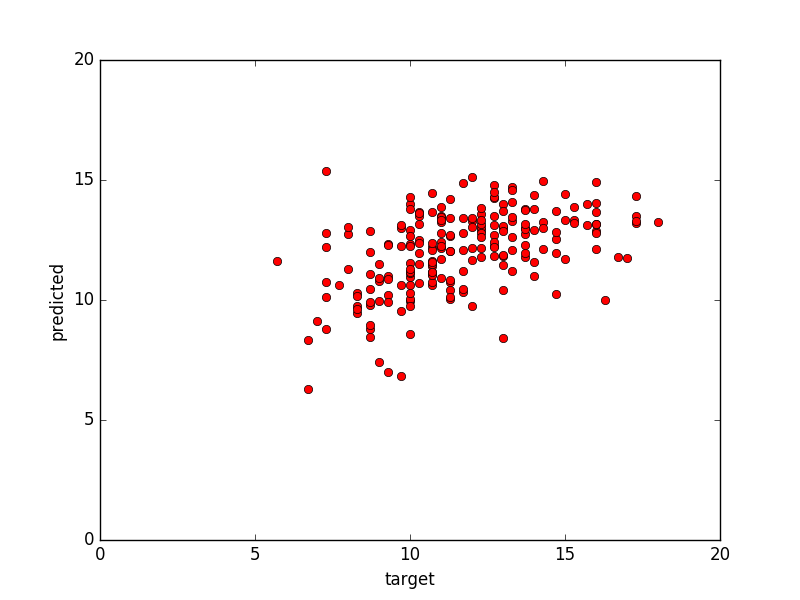
\includegraphics[width = 0.9\linewidth]{l_regression_test.png}
    \caption{Regression visualization showing predicted vs target values}
    \label{fig:fig1}
\end{figure}

\subsection{Naïve Bayes}
The implemented algorithm turned out to be unsuitable for this task as the results were not satisfactory. However, the results given by Weka were much better, probably due to slightly different implementation.

\subsubsection{Binary Classification}
For binary classification, the accuracy of our code is 63.81 \%. The accuracy of Weka's classifier is 66.19 \%.
\begin{table}[h]
\begin{center}
  \begin{tabular}{c|cc}
  & \multicolumn{2}{c}{\textbf{Target Class}} \\
 \textbf{Output} & Below & Above\\ \hline
  Below & 58 & 17 \\
  Above & 59 & 76
\end{tabular}
\quad
\begin{tabular}{c|cc}
  & \multicolumn{2}{c}{\textbf{Target Class}} \\
 \textbf{Output} & Below & Above\\ \hline
  Below & 64 & 18 \\
  Above & 53 & 75
\end{tabular}
\caption{Left table: Our Results for $k = 1$; Right table: Weka's results for $k = 2$ }
\label{tab:kNNbin}
\end{center}
\end{table}

\subsubsection{Multilevel Classification}
In multilevel classification, the accuracy of our code is only 19.52 \%, while Weka's classifier achieved the accuracy of 31.90 \%.
\begin{table}[h]
  \begin{tabular}{l|ccccc}
     & \multicolumn{5}{c}{\textbf{Target Class}} \\ 
  \textbf{Output} & Very Good & Good & Satisfactory & Sufficient & Fail \\  \hline
  Very Good  & 15 & 19 & 49 & 56 & 21\\
     Good & 0 & 2 & 2 & 0 & 0\\
     Satisfactory & 1 & 0 & 0 & 3 & 0\\
     Sufficient & 0 & 0 & 3 & 7 & 8\\
     Fail & 0 & 1 & 1 & 5 & 17\\
  \end{tabular}
  \caption{Confusion matrix of our own implementation}
  \label{tab:kNNmultiOwn}
\end{table}

\begin{table}[h]
  \begin{tabular}{l|ccccc}
     & \multicolumn{5}{c}{\textbf{Target Class}} \\ 
  \textbf{Output} & Very Good & Good & Satisfactory & Sufficient & Fail \\  \hline
  Very Good  & 2 & 2 & 6 & 5 & 0\\
     Good & 5 & 8 & 19 & 6 & 3\\
     Satisfactory & 6 & 8 & 18 & 32 & 3\\
     Sufficient & 2 & 3 & 10 & 16 & 17\\
     Fail & 1 & 1 & 2 & 12 & 23\\
  \end{tabular}
  \caption{Confusion matrix outputted by Weka's algorithm}
  \label{tab:kNNmultiWeka}
\end{table}

\subsection{k-Nearest Neighbor}
As mentioned in section 3.1. the kNN algorithm was implemented in Java and achieved similar results as the kNN algorithm provided by Weka. In this section the confusion matrices for both techniques for both classification techniques, i.e. binary and multilevel classification, are shown and compared. 
\subsubsection{Binary Classification}
For binary classification our implementation achieves the highest and equal accuracy for $ k = 1 $ and $ k = 2$. Interestingly, for both $k$ values we get the same number of 129 correctly and 81 incorrectly classified results of 210 test instances i.e. an accuracy of 61.43\%. However, the F1 scores differentiate slightly for both $k$ values with 61.3 \% for $k = 1$ and 60.7 \% for $k = 2$. \\
\\
Weka's nearest neighbor classifier performs best with $k = 2$. It classifies 137 correctly and 73 incorrectly, therefore achieving an accuracy of 65.24\% and an F1 score of 65.2\%. Table \ref{tab:kNNbin} shows the confusion matrix of our implementation for $k=1$ on the left side and Weka's confusion matrix for $k = 2$ on the right side.
\begin{table}[h]
\begin{center}
  \begin{tabular}{c|cc}
  & \multicolumn{2}{c}{\textbf{Target Class}} \\
 \textbf{Output} & Above & Below\\ \hline
  Above & 70 & 58 \\
  Below & 23 & 59
\end{tabular}
\quad
\begin{tabular}{c|cc}
  & \multicolumn{2}{c}{\textbf{Target Class}} \\
 \textbf{Output} & Above & Below\\ \hline
  Above & 55 & 35 \\
  Below & 38 & 82
\end{tabular}
\caption{Left table: Our Results for $k = 1$; Right table: Weka's results for $k = 2$ }
\label{tab:kNNbin}
\end{center}
\end{table}

\subsubsection{Multilevel Classification}
For multilevel classification our implementation achieves the highest accuracy for $ k = 1$. Out of 210 test instances 69 are classified correctly and 141 incorrectly. Thus, we achieve an accuracy of 32.86\% and a F1 score of 32.1 \%.  Weka classifies 66 instances correctly and 144 incorrectly, which results in an accuracy of 31.4\% and a F1 score of 32.4\%. Table \ref{tab:kNNmultiOwn} and \ref{tab:kNNmultiWeka} show the confusion matrix for our implementation respectively Weka.

\begin{table}[h]
  \begin{tabular}{l|ccccc}
     & \multicolumn{5}{c}{\textbf{Target Class}} \\ 
  \textbf{Output} & Very Good & Good & Satisfactory & Sufficient & Fail \\  \hline
  Very Good  & 5 & 3 & 5 & 5 & 3\\
     Good & 4 & 6 & 14 & 13 & 7\\
     Satisfactory & 4 & 6 & 23 & 22 & 8\\
     Sufficient & 2 & 5 & 8 & 18 & 11\\
     Fail & 1 & 2 & 5 & 13 & 17\\
  \end{tabular}
  \caption{Confusion matrix of our own kNN implementation}
  \label{tab:kNNmultiOwn}
\end{table}

\begin{table}[h]
  \begin{tabular}{l|ccccc}
     & \multicolumn{5}{c}{\textbf{Target Class}} \\ 
  \textbf{Output} & Very Good & Good & Satisfactory & Sufficient & Fail \\  \hline
  Very Good  & 3 & 5 & 5 & 5 & 0\\
     Good & 5 & 6 & 14 & 9 & 8\\
     Satisfactory & 6 & 6 & 21 & 25 & 9\\
     Sufficient & 2 & 4 & 8 & 22 & 15\\
     Fail & 0 & 1 & 7 & 10 & 14\\
  \end{tabular}
  \caption{Confusion matrix outputted by Weka's kNN algorithm}
  \label{tab:kNNmultiWeka}
\end{table}

\subsection{Artificial Neural Networks for Regression}
ANN performing regression was implemented in Python with use of TensorFlow library. Multi-Layer Perceptron architecture was chosen, with 3 hidden layers, each layer containing 15 neurons with rectifier activation function. For training, Adam Optimizer algorithm minimizing mean square error cost function was used. The learning rate was set to 0.001 and number of epochs to 4000, as beyond that point, network was sensitive to overfitting.

As Weka doesn't support specifying the learning algorithm, it can't be directly compared and different parameters had to be selected. The best result was achieved with learning rate 0.01, momentum 0.2 and training for 500 epochs.

\begin{table}[h!]
  \centering
  \begin{tabular}{lll}
  \hline
 \textbf{Metric} & \textbf{TensorFlow} & \textbf{Weka} \\ \hline
  Mean Square Error & 4.97 & 5.52 \\
  Mean Absolute Error & 1.76 & 1.87\\
  Relative Absolute Error & 85.86 \% & 91.17 \%\\
  \hline
  \end{tabular}
  \caption{Regression results for ANN}
  \label{tab:table2}
\end{table}

\begin{figure}[h!]
    \centering
    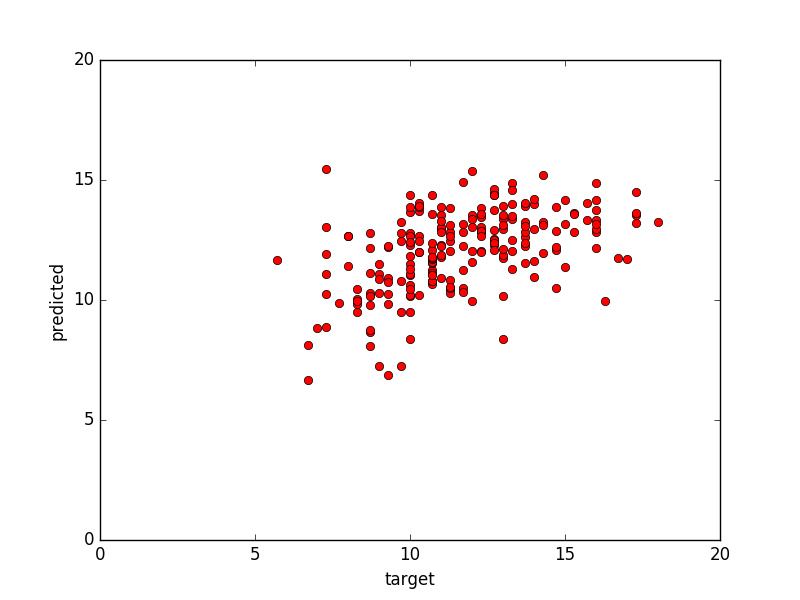
\includegraphics[width = 0.9\linewidth]{regression_test.png}
    \caption{Regression visualization showing predicted vs target values}
    \label{fig:fig1}
\end{figure}


\subsection{Artificial Neural Networks for Classification}
As previously mentioned, the classification part of the ANN implementation was done in Matlab, using its Pattern Recognition tool. Scaled conjugate gradient backpropagation was used as the learning algorithm, which tried to minimize the cross-entropy error. The multilayer perceptron neural network (MLP) had one hidden layer with 10 hidden neurons.

The following four tables show the results for the four tests. The first two tables include the confusion matrices from Matlab, while the second two tables contain the confusion matrices from Weka. 

\begin{table}[h!]
  \centering
  \begin{tabular}{l|cccccc}
     & \multicolumn{5}{c}{\textbf{Target Class}} \\ 
    \textbf{Output} & Fail & Sufficient & Satisfactory & Good & Very Good\\
    \hline
    Fail & 1 & 0 & 1 & 0 & 0\\ 
    Sufficient & 1 & 3 & 2 & 2 & 0\\ 
    Satisfactory & 22 & 34 & 73 & 47 & 24\\  
    Good & 20 & 49 & 82 & 98 & 49\\  
    Very Good & 3 & 4 & 10 & 40 & 69\\
  \end{tabular}
  \caption{Matlab implementation's confusion matrix for the 5-class problem.}
  \label{tab:table1}
\end{table}



\begin{table}[h!]
  \centering
  \begin{tabular}{c|cc}
    & \multicolumn{2}{c}{\textbf{Target Class}} \\ 
    \textbf{Output} & Below & Above \\ \hline 
     Below & 227 & 57\\ 
     Above & 102 & 248\\ 
  \end{tabular}
  \quad
  \begin{tabular}{c|cc}
    & \multicolumn{2}{c}{\textbf{Target Class}} \\
    \textbf{Output} & Below & Above\\ \hline
    Below & 244 & 95  \\
    Above & 85 & 210 \\
  \end{tabular}
  
  \caption{Left Table: Matlab implementation's confusion matrix for the binary problem. Right Table: Weka implementation's confusion matrix for the binary problem.}
  \label{tab:table1}
\end{table}

In Weka, the MLPClassify classifier function was used to perform the classifications. The following are the tables of classifications collected.

\begin{table}[h!]
  \centering
  \begin{tabular}{l|ccccc}
    & \multicolumn{5}{c}{\textbf{Target Class}} \\
    \textbf{Output} & Fail & Sufficient & Satisfactory & Good & Very Good\\ \hline
    Fail & 44 & 41 & 16 & 13 & 6\\
    Sufficient & 40 & 63 & 51 & 25 & 16\\
    Satisfactory & 18 & 50 & 58 & 38 & 25\\
    Good & 6 & 25 & 27 & 18 & 6\\
    Very Good & 8 & 11 & 17 & 6 & 6\\
  \end{tabular}
  \caption{Weka implementation's confusion matrix for the 5-class problem.}
  \label{tab:table1}
\end{table}

\begin{table}[h!]
  \centering
  \begin{tabular}{ccc}
  \hline
    \textbf{Implementation} & \textbf{5-class} & \textbf{Binary} \\
    \hline
    Matlab &  38.5 \%  & 74.8 \%  \\
    Weka  & 29.8 \% & 71.6 \%  \\
    \hline
  \end{tabular}
  \caption{Classification Accuracies for ANN Classification}
  \label{tab:table1}
\end{table}

\subsection{Decision Trees}

The decision trees were implemented both in Python using the sklearn library, and in Weka. The results and confusion matrices of these implementations are presented and compared in this section.

\subsubsection{Binary Classification}
For the binary classification, the Python sklearn classification was more accurate than the Weka implementation with 68.1 \% and 63.3 \% precision respectively. The confusion matrices are shown in table \ref{tab:DTbinary}.

\begin{table}[h]
\begin{center}
  \begin{tabular}{c|cc}
  & \multicolumn{2}{c}{\textbf{Target Class}} \\
 \textbf{Output} & Above & Below\\ \hline
  Above & 79 & 38 \\
  Below & 29 & 64
\end{tabular}
\quad
\begin{tabular}{c|cc}
  & \multicolumn{2}{c}{\textbf{Target Class}} \\
 \textbf{Output} & Above & Below\\ \hline
  Above & 64 & 53 \\
  Below & 24 & 69
\end{tabular}
\caption{Left table: Confusion matrix of sklearn implementation; Right table: Confusion matrix of Weka implementation }
\label{tab:DTbinary}
\end{center}
\end{table}

\subsubsection{Multilevel Classification}
For the 5-level classification, the sklearn implementation again achieved the best result with 33.8 \% accuracy, compared to the 31 \% accuracy of the Weka implementation. The confusion matrices of the sklean and Weka classifiers are shown in table \ref{tab:DT5level_sklearn} and \ref{tab:DT5level_weka} respectively.

\begin{table}[h]
  \begin{tabular}{l|ccccc}
     & \multicolumn{5}{c}{\textbf{Target Class}} \\ 
  \textbf{Output} & Very Good & Good & Satisfactory & Sufficient & Fail \\  \hline
  Very Good  & 5 & 3 & 4 & 3 & 1\\
     Good & 2 & 7 & 5 & 6 & 2\\
     Satisfactory & 8 & 16 & 15 & 12 & 4\\
     Sufficient & 5 & 9 & 18 & 25 & 14\\
     Fail & 2 & 7 & 8 & 10 & 19\\
  \end{tabular}
  \caption{Confusion matrix of sklearn implementation}
\label{tab:DT5level_sklearn}
\end{table}

\begin{table}[h]
  \begin{tabular}{l|ccccc}
     & \multicolumn{5}{c}{\textbf{Target Class}} \\ 
  \textbf{Output} & Very Good & Good & Satisfactory & Sufficient & Fail \\  \hline
  Very Good  & 1 & 4 & 8 & 2 & 1\\
     Good & 3 & 5 & 9 & 4 & 1\\
     Satisfactory & 7 & 19 & 16 & 7 & 6\\
     Sufficient & 5 & 13 & 16 & 20 & 17\\
     Fail & 1 & 3 & 7 & 12 & 23\\
  \end{tabular}
  \caption{Confusion matrix of Weka implementation}
\label{tab:DT5level_weka}
\end{table}

\subsection{Comparison of all algorithms and discussion of results}
Across the experiment, binary and five-class classifiers were successfully built for the dataset. However, classification accuracy of over 75\% on the binary classifier, and over 40\% on the five-class classifier was not achieved, as shown in table \ref{tab:ClassificationAccuracy}.\\

\begin {table}[h]
\begin{center}
  \begin{tabular}{lllll}  
    \hline
   \textbf{Classification} & \textbf{ANN} & \textbf{kNN} & \textbf{DT} \\ \hline
    5-class & 38.5 \% & 33 \% & 34 \% \\
    binary & 74.8 \% & 61 \% & 68 \% \\
    \hline
  \end{tabular}
  \caption{Classification Accuracy}
 \label{tab:ClassificationAccuracy}
\end{center}
\end{table}

As can be expected from these results, none of these algorithms can make perfect (or probably even reliable) classifications or regressions from the data set. Among the three algorithms, the artificial neural network proved to be the most accurate, with a five-class of 38.5\% and a binary reaching almost 75\%. Referring back to the inividual discussion of each algorithm, with all of the from-scratch implementations of the algorithms explored, it can be found that each one reaches conclusions relatively close to that found by the Weka implementations. This closeness in results reveals that the algorithms implemented may be sufficient and reliable under normal circumstances, and show that the lack of accuracy in classification can be found in other areas.

This aforementioned lack of accuracy can most likely be found in the sourced data set itself. This may be due to:
    \begin{itemize}
        \item The data set not being big enough (649 records). Simply put, more students need to be gathered for this set.
        \item The data set features not having a large enough influence on the classes, more specifically an attribute cannot reliably contribute towards the classification of a student.
        \item The attributes used in this data set may not have been the best in terms of accurately relating to student performance.
        \item The timespan of data collected may not be broad enough: only one school year was covered in two public schools. This may be rectified by sourcing data across multiple school years or gathering data from across the region.
    \end{itemize}  
